
\begin{figure}[] % t 表示放在页首，也可以用 htbp
\vspace{-27pt}
  \centering
  % 第一张子图，宽度设为单行总宽度的 32%
  \begin{subfigure}[b]{0.32\textwidth}
    \centering
    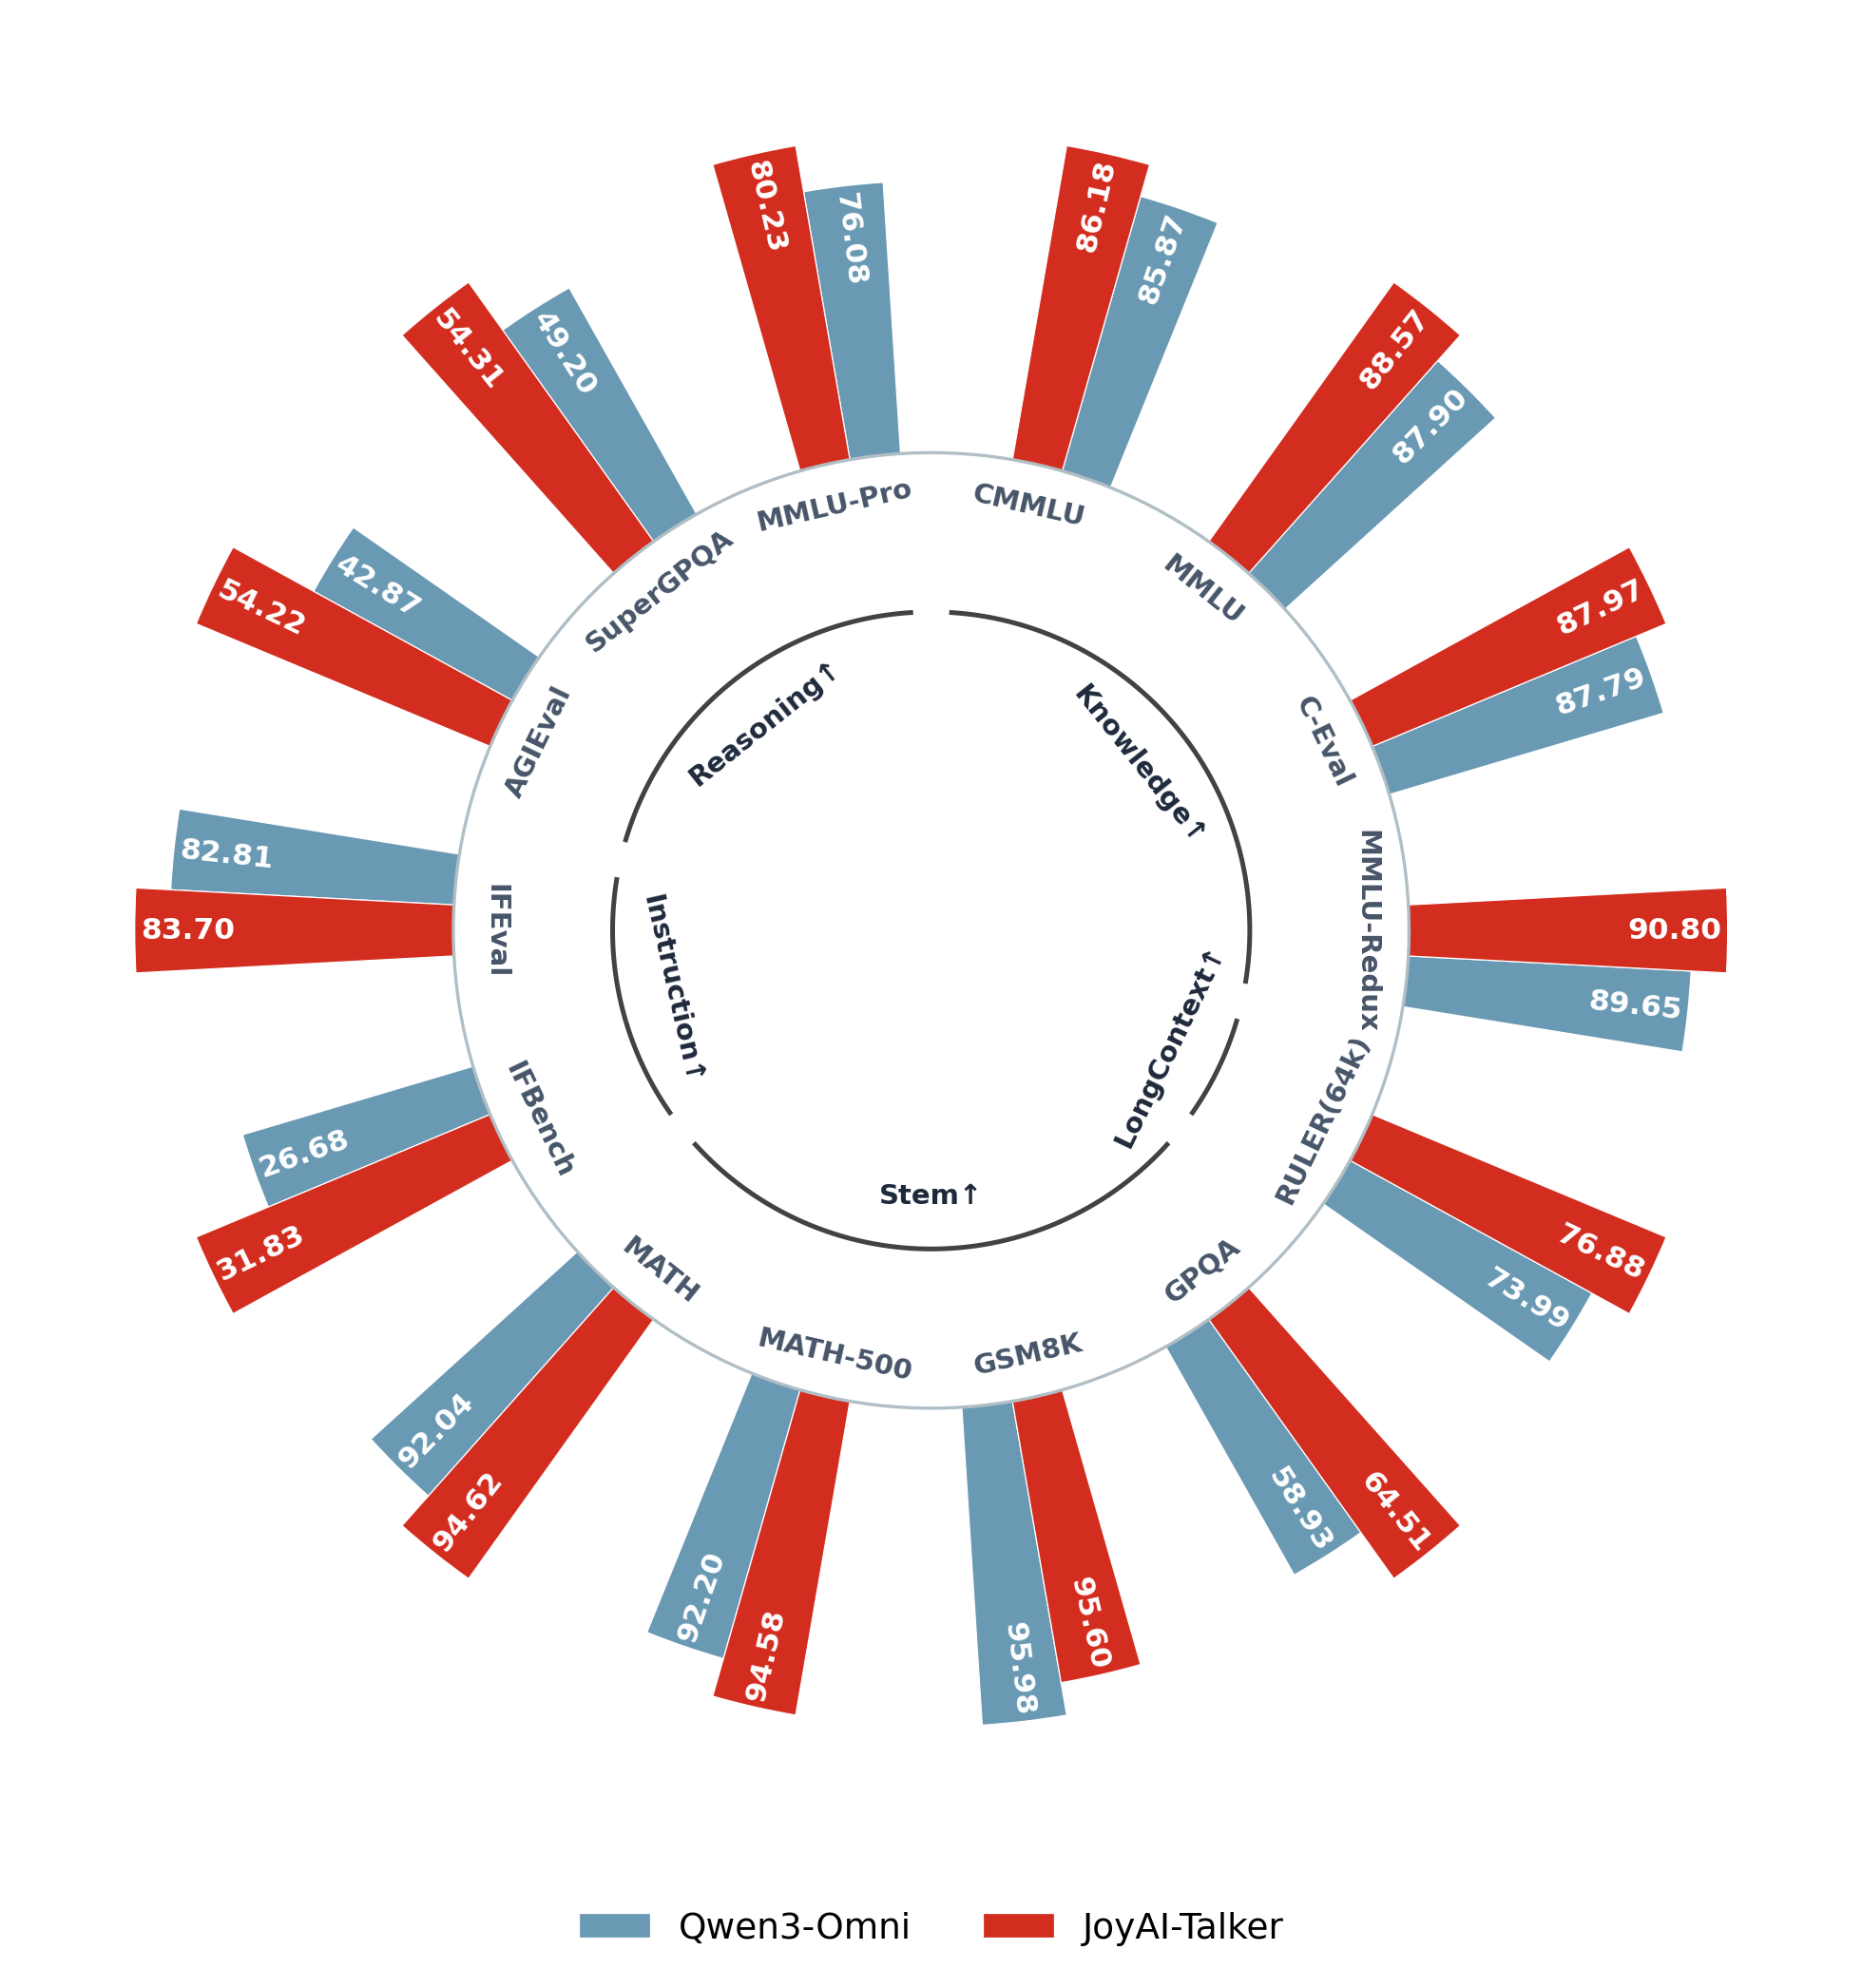
\includegraphics[width=\textwidth]{pic/T2T.png} % 替换为您的图片路径
    \vspace{-15pt}
    \caption{T2T} % 子图a的标题
    \label{fig:sub_a} % 子图a的引用标签
  \end{subfigure}
  \hfill % 自动分配中间的水平间距
  % 第二张子图
  \begin{subfigure}[b]{0.32\textwidth}
    \centering
    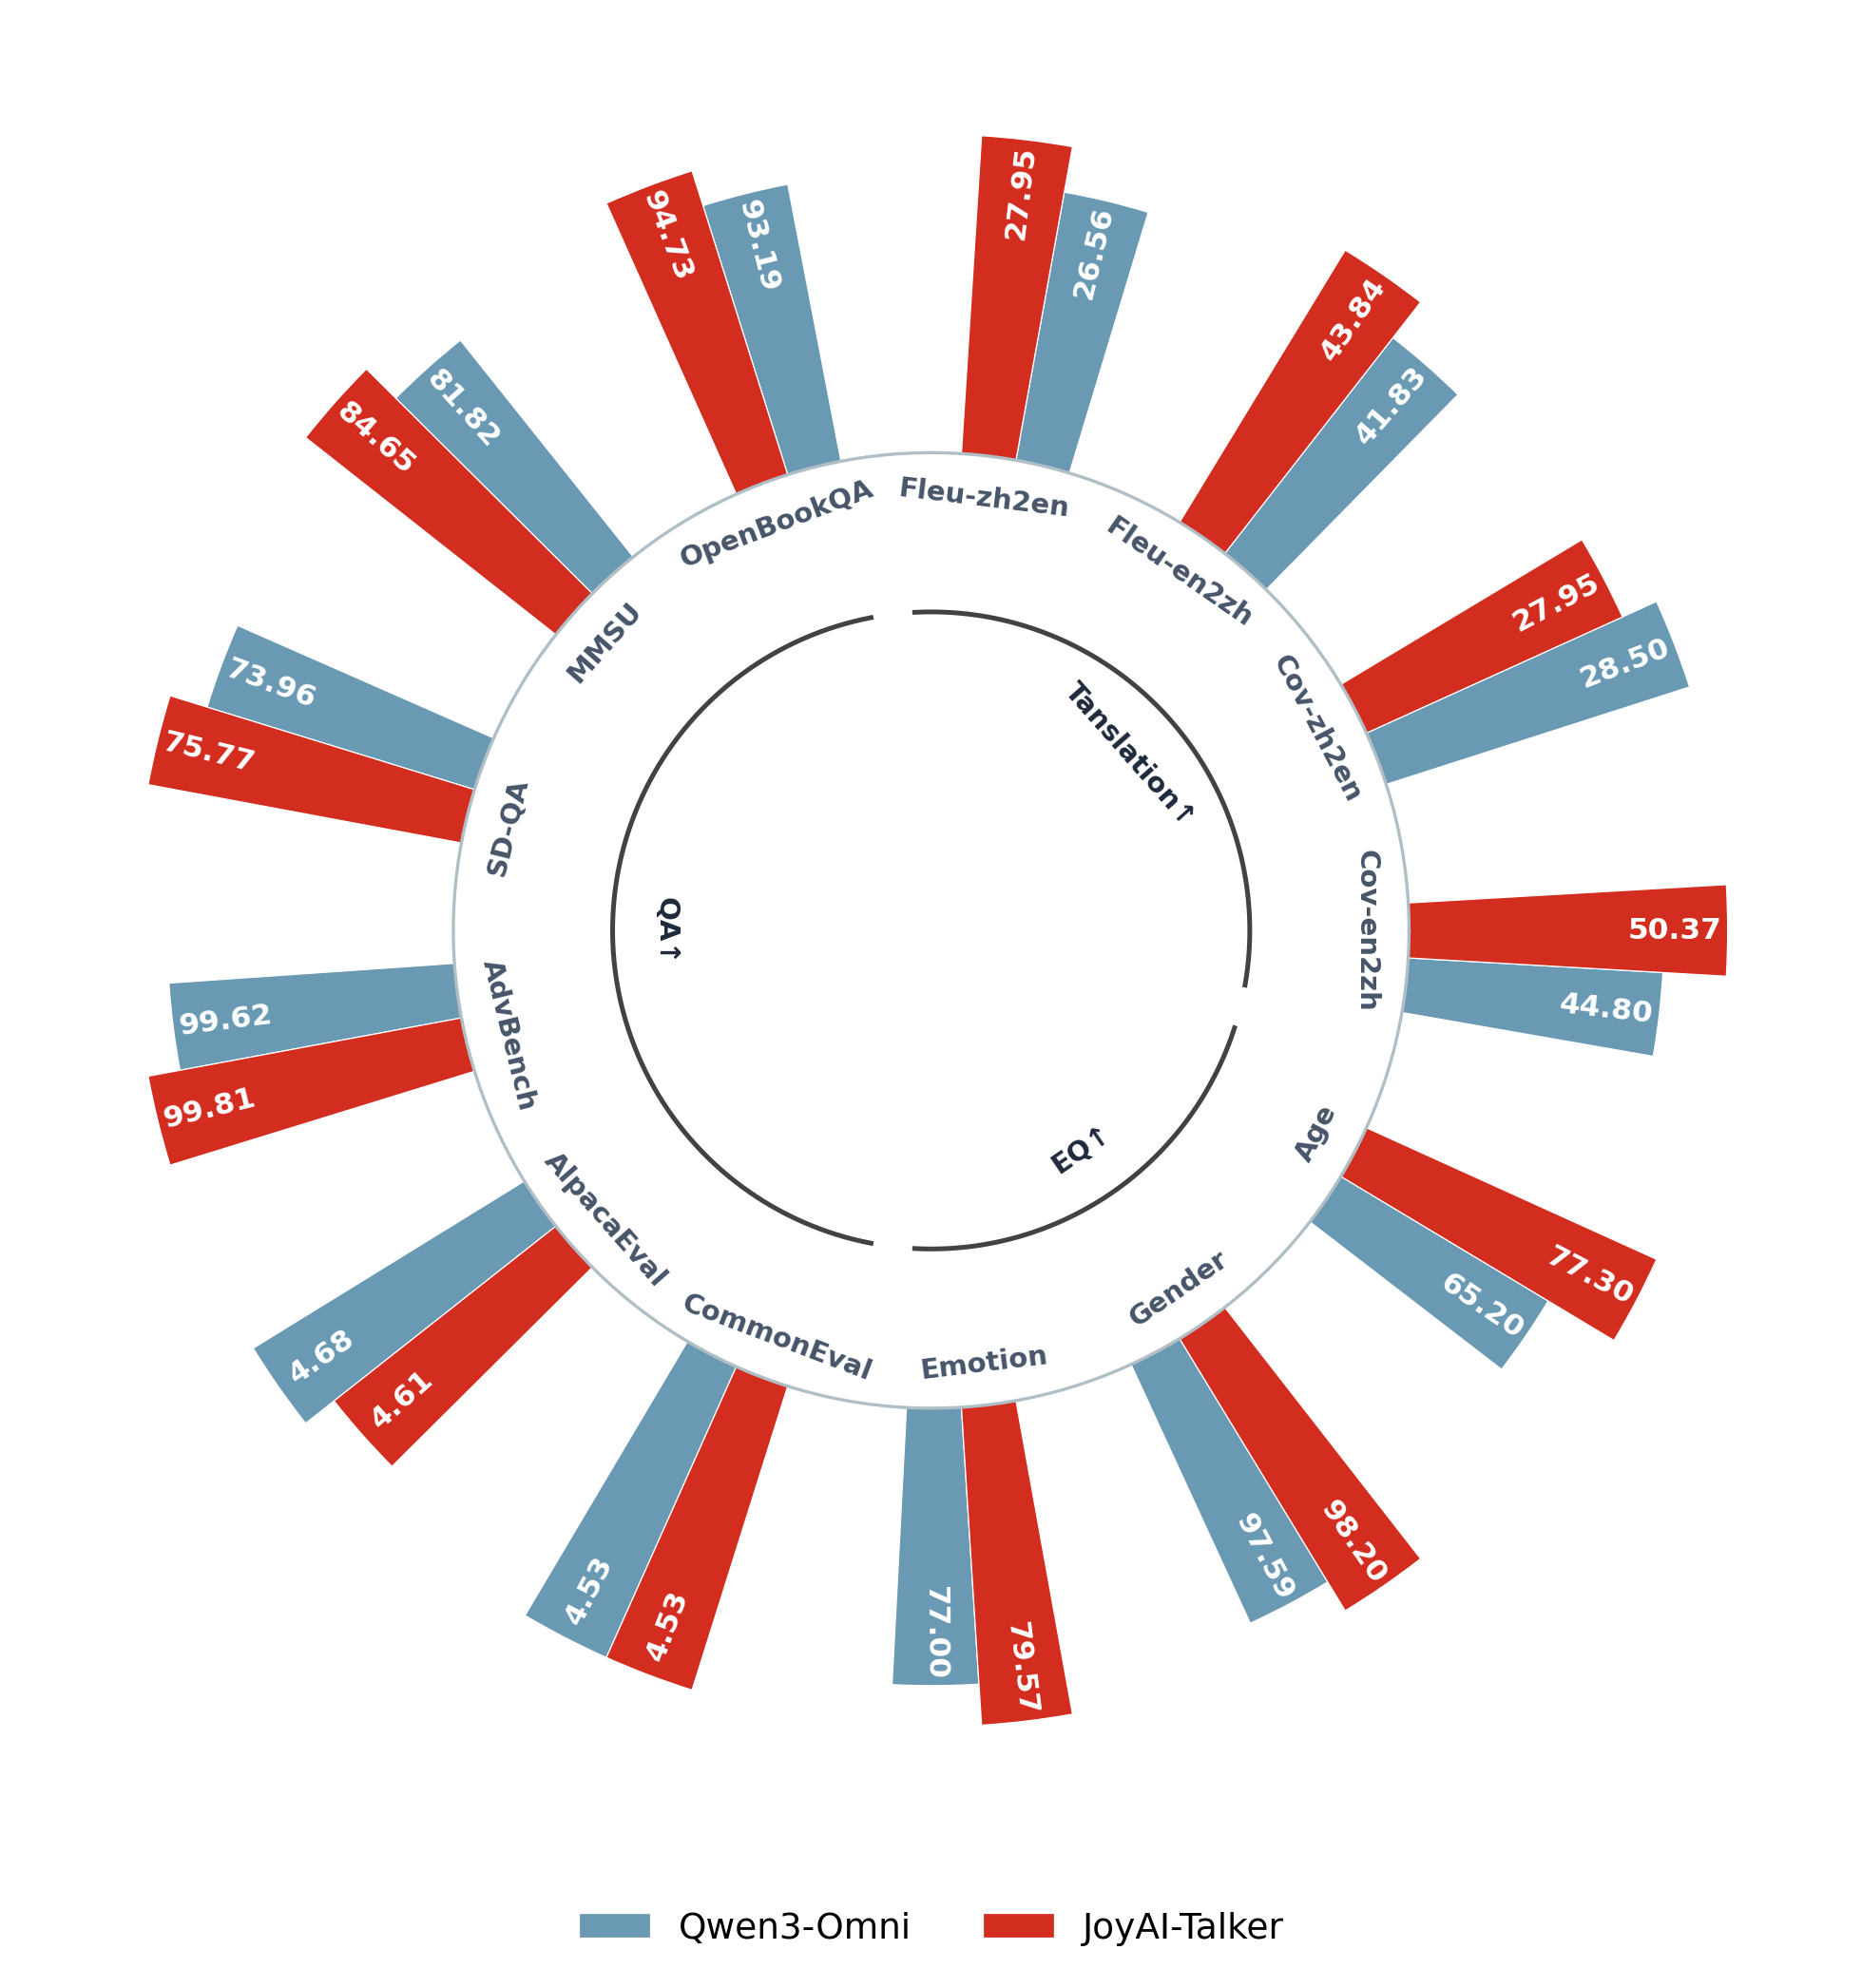
\includegraphics[width=\textwidth]{pic/S2T-QA.png}
    \vspace{-15pt}
    \caption{S2T - QA, Tanslation, EQ} % 子图b的标题
    \label{fig:sub_b}
  \end{subfigure}
  \hfill % 自动分配中间的水平间距
  % 第三张子图
  \begin{subfigure}[b]{0.32\textwidth}
    \centering
    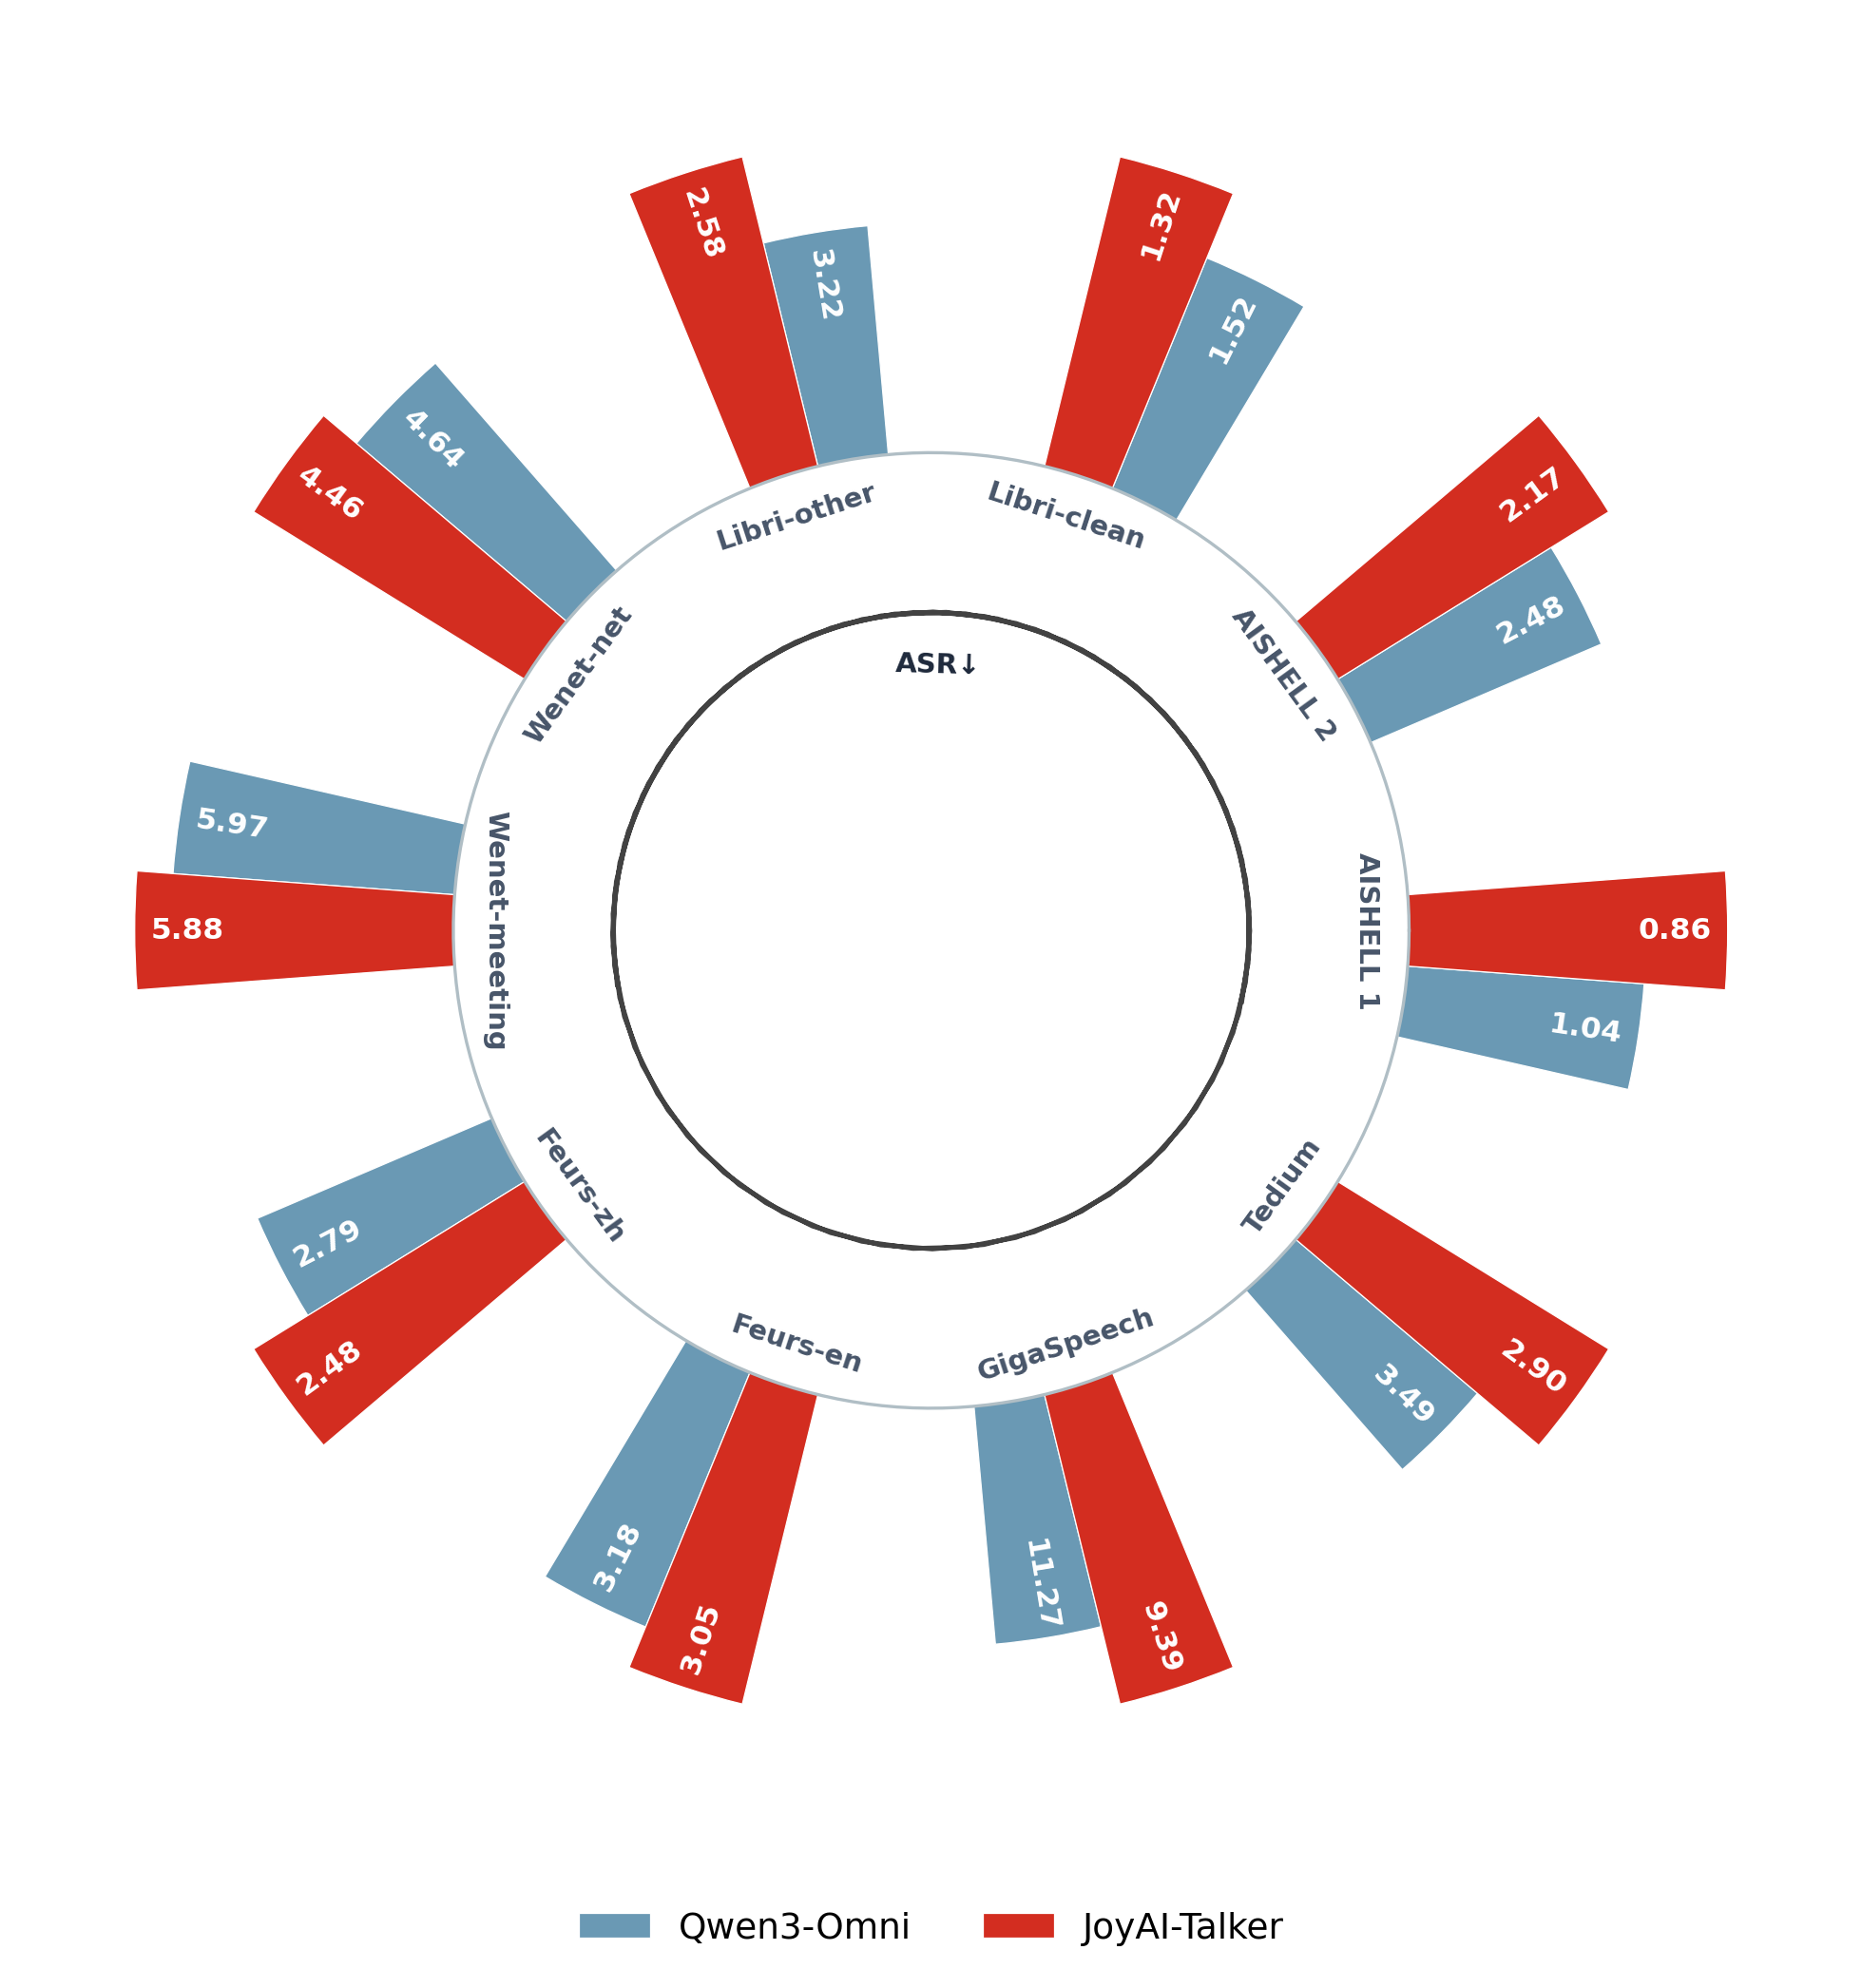
\includegraphics[width=\textwidth]{pic/S2T-ASR.png}
    \vspace{-15pt}
    \caption{S2T - ASR} % 子图c的标题
    \label{fig:sub_c}
  \end{subfigure}
  % 主图的大标题
  \vspace{-8pt}
  \caption{Overall performance of JoyAI-Talker across T2T and S2T benchmark.}
  \label{fig:main_figure} % 主图引用标签
\end{figure}

\section{Introduction}
\label{sec:introduction}

The rapid advancement of Large Language Models (LLMs) has profoundly accelerated the development of intelligent conversational agents. However, since speech remains the most natural, expressive, and efficient modality for human communication, the research paradigm is increasingly shifting from text-centric models toward Large Speech Language Models (LSLMs). Historically, speech dialogue systems relied on cascaded architectures—comprising Automatic Speech Recognition (ASR), an LLM, and Text-to-Speech (TTS) modules. While functional, these pipelines suffer from compounded latency and the irreversible loss of rich paralinguistic cues (e.g., emotion, intonation, and hesitation) during the text-bottleneck conversion. Recently, the industry has witnessed a breakthrough in end-to-end multi-modal architectures. Advanced proprietary models, such as GPT-4o and Gemini 3.1 Live, have pushed the boundaries of real-time, highly expressive voice interactions. Concurrently, open-weight pioneers like Moshi~\cite{defossez2024moshi}, Freeze-Omni~\cite{freezeomni2024}, and Qwen3-Omni~\cite{qwen3omni2025} have explored various dual-stream or natively unified structures to achieve lower latency and richer acoustics. Despite these unprecedented strides, achieving truly human-like, immersive, and intelligent conversational agents still faces three fundamental challenges:


\begin{itemize}
    \item \textbf{Modality-Induced Cognitive Degradation:} Integrating the continuous, high-dimensional speech modality into the discrete linguistic space of LLMs often triggers ``catastrophic forgetting.'' During joint multi-modal training, models typically sacrifice their foundational logical reasoning, mathematical proficiency, and complex problem-solving capabilities, forcing a suboptimal trade-off between textual intelligence and acoustic alignment.
    
    \item \textbf{Lack of Dynamic and Contextual Empathy:} Current voice assistants tend to generate flat, generalized responses. While some models can simulate basic emotions, they struggle to dynamically perceive fine-grained speaker attributes (e.g., age, gender, and underlying emotional states) from the input audio. Intertwining logical reasoning with rich paralinguistic behaviors (e.g., laughter, sighs, and hesitations) remains difficult, making it challenging to deliver the customized, empathetic interactions characteristic of genuine human communication.
    
    \item \textbf{Fragile Full-Duplex Interaction:} Real-world conversations are highly unstructured, filled with overlaps, backchannels, and ambient noise. Traditional full-duplex systems~\cite{defossez2024moshi} or energy-based Voice Activity Detection (VAD) methods suffer from high false activation rates. As observed in recent benchmarks~\cite{lin2026fullduplexv1.5}, speech dialogue agents tend to adopt extreme policies: they are either over-reactive (triggering heavily on background noise and interruptions) or over-conservative (failing to yield during genuine user speech), thereby disrupting the natural conversational flow.
\end{itemize}




To address these critical bottlenecks, we introduce \textbf{JoyAI-Talker}, a full-duplex speech dialogue system that delivers expressive, empathetic, and stable real-time full-duplex interactions. JoyAI-Talker adopts an innovative, decoupled \textbf{Duplex-Thinker--Talker} architecture. The language backbone is built upon JoyAI-LLM Flash~\cite{cai2026joyaillmflashadvancingmidscale}, a 48.9B-parameter sparse Mixture-of-Experts (MoE) model featuring Multi-Head Latent Attention (MLA) and auxiliary-loss-free routing, inspired by recent large-scale MoE architectures such as DeepSeek-V3~\cite{deepseekai2025deepseekv3technicalreport} and Kimi-K2~\cite{kimiteam2026kimik2openagentic}. The \textit{Thinker} focuses on acoustic understanding, empathetic reasoning, and response formulation, while the \textit{Talker}—which follows the speech generation architecture of JoyVoice~\cite{joyvoice}—acts as a controllable, low-latency speech generator capable of interpreting natural-language instructions and explicit paralinguistic tokens.



The key features and capabilities of JoyAI-Talker are summarized as follows:

\begin{itemize}
    \item \textbf{Foundational Capability for Conversational Voice Agents:} 
    Instead of functioning as a narrow interaction model, JoyAI-Talker is developed as a highly versatile foundation model that delivers competitive performance across a diverse range of cognitive, reasoning, and linguistic benchmarks. By maintaining a unified semantic and acoustic modeling interface, the system simultaneously provides a robust, extensible base to support conversational voice agents, enabling multi-turn speech reasoning and tool-use.
    
    \item \textbf{Unified Joint Training with Alleviated Cognitive Degradation:} 
    Rather than delaying speech-text integration until the post-training phase, we adopt a unified speech-text joint training paradigm starting from the early mid-training phase. By carrying this joint modeling through Mid-training, Context Extension, SFT, and DPO, JoyAI-Talker alleviates the common "cognitive degradation" bottleneck to a certain extent. The model preserves its fundamental reasoning, STEM, and logical capabilities in the textual domain (e.g., reaching 94.62\% on MATH), demonstrating a favorable balance between text-based intelligence and speech interaction.
    
    \item \textbf{Persona-Adaptive Empathetic Response (PAER) via CoT:} 
    We introduce a progressive cognitive empathy framework structured as a hierarchical pipeline: audio understanding $\rightarrow$ Chain-of-Thought (CoT) reasoning $\rightarrow$ empathetic dialogue generation. Guided by this pipeline, the Thinker first extracts speaker attributes—such as gender, age, and emotional state—from the raw input audio. It then integrates these perceived attributes into its CoT reasoning to formulate context-adaptive responses. These responses combine semantically appropriate text with precise, token-level controls over utterance-level expressions (e.g., speaking rate and volume) and localized paralinguistic events, allowing the Talker to deliver expressive, personalized speech while maintaining a consistent assistant identity.
    
    \item \textbf{Decoupled, Text-Controllable Expressive Speech Generation:} 
    The Talker module employs a decoupled, instruction-controllable speech generation paradigm to translate semantic outputs and speaking instructions into speaker-consistent, expressive speech. By separating response planning from acoustic execution, the Talker dynamically controls prosody, emotional expression, and localized paralinguistic behaviors (e.g., \texttt{[Laughter]} and \texttt{[Sigh]}) via natural-language instructions and explicit vocabulary tokens, while maintaining a stable assistant identity.
    
    \item \textbf{Joy-Duplex: A Non-Intrusive, Highly Stable Full-Duplex Framework:} 
    Departing from computationally heavy end-to-end parallel dual-stream architectures, we propose a modular, state-driven, plug-and-play full-duplex framework. By integrating fine-grained interaction state tokens directly into the streaming decoding path, Joy-Duplex serves as an efficient gating engine for real-time turn control. On the rigorous Full-Duplex-Bench v1.5~\cite{lin2026fullduplexv1.5}, Joy-Duplex delivers a well-balanced interaction policy, achieving a high responsiveness of 0.88 under user interruptions while keeping false triggers extremely low under background speech, representing a robust and stable interaction policy for fluid speech dialogue.
\end{itemize}